% !TeX spellcheck = fr_FR
\chapter{Chapitre 12 : Dockerisation and repo files}

Ce chapitre raconte la « vie en conteneurs » de notre projet. Objectif: en une commande, tout démarre, la base de données se prépare, les scripts s'enchaînent, et l'application web apparaît sur \texttt{http://localhost:5001}. Nous allons décortiquer la configuration, illustrer les choix et montrer des extraits utiles.

\medskip
\noindent\textbf{On verra} comment fonctionnent \texttt{dockerfile}, \texttt{docker-compose.yml}, \texttt{entrypoint.sh} et \texttt{.dockerignore} ensemble; comment lancer le pipeline complet ou un mode \textit{dev} léger; et comment diagnostiquer, personnaliser et améliorer l'ensemble.

\section{Pourquoi dockeriser ?}

Trois raisons concrètes :
\begin{itemize}
  \item \textbf{Reproductibilité}: même version de Python, mêmes dépendances système (\texttt{wkhtmltopdf}, client MySQL), même environnement d'exécution.
  \item \textbf{Parité dev/prod}: une pile unique (app + base) réduisant les \og ça marche sur ma machine\fg{}.
  \item \textbf{Bootstrap instantané}: une commande pour installer, migrer, télécharger/traiter les données et lancer le serveur.
\end{itemize}

\section{Les quatre pièces du puzzle}

\begin{description}
  \item[\texttt{dockerfile}] Image de l'application: base Python 3.9 \texttt{slim-bookworm}, dépendances \textit{apt}, \texttt{pip}, copie du code et \texttt{ENTRYPOINT}.
  \item[\texttt{docker-compose.yml}] Orchestration multi-services: \texttt{db} (MySQL) + \texttt{app} et \texttt{app-dev} (profils), volumes, variables d'environnement, \texttt{depends\_on} avec healthcheck.
  \item[\texttt{entrypoint.sh}] Orchestrateur de démarrage côté \texttt{app}: attend MySQL, applique migrations, exécute scripts de données (selon flags), lance Flask.
  \item[\texttt{.dockerignore}] Réduit le contexte de build (ignore les dossiers volumineux et la documentation), accélère et assainit l'image.
\end{description}

\section{Aperçu}

\begin{figure}[H]
  \centering
  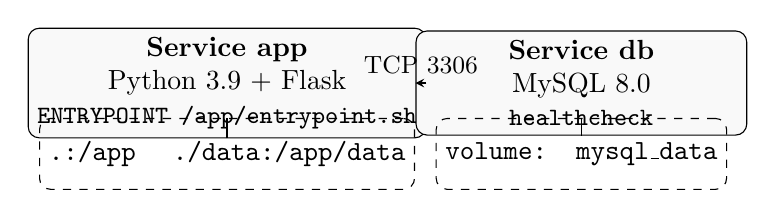
\begin{tikzpicture}[node distance=1.8cm, >=stealth]
    \tikzstyle{svc}=[draw, rounded corners, minimum width=4.2cm, minimum height=1.2cm, align=center, fill=gray!5]
    \tikzstyle{vol}=[draw, dashed, rounded corners, minimum width=3.5cm, minimum height=0.9cm, align=center]

    \node[svc] (app) {\textbf{Service app}\\ Python 3.9 + Flask\\ \small \texttt{ENTRYPOINT /app/entrypoint.sh}};
    \node[svc, right of=app, node distance=4.5cm] (db) {\textbf{Service db}\\ MySQL 8.0\\ \small \texttt{healthcheck}};
    \node[vol, below of=db, node distance=0.9cm] (mysqlvol) {\texttt{volume: mysql\_data}};
    \node[vol, below of=app, node distance=0.9cm] (codevol) {\texttt{.:/app} \quad \texttt{./data:/app/data}};

    \draw[->] (app) -- node[above]{\small TCP 3306} (db);
    \draw[-] (db) -- (mysqlvol);
    \draw[-] (app) -- (codevol);
  \end{tikzpicture}
  \caption{Deux conteneurs reliés sur le réseau compose; volumes pour le code (monté) et les données MySQL (persistées).}
\end{figure}

\section{L'orchestration: \texttt{docker-compose.yml}}

Le fichier compose définit \texttt{db}, \texttt{app} et un service \texttt{app-dev} activé via profil. Extraits commentés:

\begin{codebox}{\texttt{db} : MySQL 8.0 avec healthcheck}
services:
  db:
    image: mysql:8.0
    environment:
      MYSQL_ROOT_PASSWORD: root
      MYSQL_DATABASE: stops_db
      MYSQL_USER: stops_user
      MYSQL_PASSWORD: 1234
    ports:
      - "3306:3306"
    volumes:
      - mysql_data:/var/lib/mysql
    healthcheck:
      test: ["CMD-SHELL", "mysqladmin ping -h localhost -u$${MYSQL_USER} -p$${MYSQL_PASSWORD}"]
      interval: 10s
      timeout: 5s
      retries: 2
\end{codebox}

\noindent L'application dépend explicitement du statut \textit{healthy} de MySQL et monte deux volumes (code + données):

\begin{codebox}{\texttt{app} : service principal}
  app:
    build: .
    ports:
      - "5001:5001"
    volumes:
      - .:/app
      - ./data:/app/data
    depends_on:
      db:
        condition: service_healthy
    environment:
      # Variables lues depuis .env si présentes (avec valeurs par défaut)
      MYSQL_USER: ${MYSQL_USER:-stops_user}
      MYSQL_PASSWORD: ${MYSQL_PASSWORD:-1234}
      AUTH_DB_USER: ${AUTH_DB_USER:-}
      AUTH_DB_PASSWORD: ${AUTH_DB_PASSWORD:-}
      DATABASE_URI: ${DATABASE_URI:-mysql+pymysql://stops_user:1234@db/stops_db}
      AUTH_DATABASE_URI: ${AUTH_DATABASE_URI:-mysql+pymysql://stops_user:1234@db/auth_db}
      AUTO_MIGRATE: "true"
      MATCH_ONLY: "${MATCH_ONLY:-false}"
      SECRET_KEY: ${SECRET_KEY:-dev-insecure}
\end{codebox}

\noindent En développement, nous activons un service plus léger qui évite les téléchargements et prétraitements longs:

\begin{codebox}{\texttt{app-dev} : profil \texttt{dev}}
  app-dev:
    profiles: [dev]
    build: .
    volumes:
      - .:/app
      - ./data:/app/data
    environment:
      SKIP_DATA_IMPORT: "true"
      AUTO_MIGRATE: "true"
\end{codebox}

\section{L'image: \texttt{dockerfile}}

L'image part d'un Python 3.9 minimal \texttt{slim-bookworm} (compatibilité \texttt{wkhtmltopdf}). Nous installons trois dépendances \textit{apt}: \texttt{wkhtmltopdf}, \texttt{default-mysql-client} (pour \texttt{mysqladmin}) et \texttt{dos2unix}. Puis \texttt{pip install -r requirements.txt} et utilisation d'un \texttt{ENTRYPOINT} shell.

\begin{codebox}[language=bash]{Extraits — \texttt{dockerfile}}
FROM python:3.9-slim-bookworm
ENV FLASK_APP=backend/app.py \\
    FLASK_RUN_HOST=0.0.0.0 \\
    FLASK_RUN_PORT=5001
RUN apt-get update && apt-get install -y --no-install-recommends \\
    wkhtmltopdf default-mysql-client dos2unix && rm -rf /var/lib/apt/lists/*
WORKDIR /app
COPY requirements.txt /app/
RUN pip install --no-cache-dir -r requirements.txt
COPY entrypoint.sh /app/entrypoint.sh
RUN dos2unix /app/entrypoint.sh && chmod +x /app/entrypoint.sh
COPY . /app/
EXPOSE 5001
ENTRYPOINT ["/bin/bash", "/app/entrypoint.sh"]
\end{codebox}

\section{Le chef d'orchestre: \texttt{entrypoint.sh}}

Le script d'entrée synchronise le démarrage: attend MySQL, crée la base \texttt{auth\_db} si besoin, applique les migrations, exécute les scripts de données (selon les drapeaux), puis lance Flask. Il peut également créer un utilisateur dédié pour \texttt{auth\_db} si des variables d'environnement sont fournies.

\begin{codebox}[language=bash]{Attente active, création de comptes, migrations}
echo "Waiting for MySQL database at db:3306..."
while ! mysqladmin ping -h"db" -P3306 --silent \\
        --user=${MYSQL_USER} --password=${MYSQL_PASSWORD}; do
    sleep 1
done
echo "MySQL is up and ready."

if [ -n "$MYSQL_ROOT_PASSWORD" ]; then
  # Assure l'existence de auth_db et droits de base
  mysql -h db -uroot -p"${MYSQL_ROOT_PASSWORD}" \\
    -e "CREATE DATABASE IF NOT EXISTS auth_db CHARACTER SET utf8mb4 COLLATE utf8mb4_unicode_ci; GRANT ALL PRIVILEGES ON auth_db.* TO 'stops_user'@'%'; FLUSH PRIVILEGES;" || true
  # Crée un utilisateur dédié auth si variables fournies et révoque stops_user sur auth_db
  if [ -n "$AUTH_DB_USER" ] && [ -n "$AUTH_DB_PASSWORD" ]; then
    mysql -h db -uroot -p"${MYSQL_ROOT_PASSWORD}" \\
      -e "CREATE USER IF NOT EXISTS '${AUTH_DB_USER}'@'%' IDENTIFIED BY '${AUTH_DB_PASSWORD}'; GRANT SELECT, INSERT, UPDATE, DELETE, CREATE, ALTER, INDEX ON auth_db.* TO '${AUTH_DB_USER}'@'%'; REVOKE ALL PRIVILEGES ON auth_db.* FROM 'stops_user'@'%'; FLUSH PRIVILEGES;" || true
  fi
fi

if [ "${AUTO_MIGRATE:-false}" = "true" ]; then
  [ ! -d "migrations" ] && flask db init || true
  flask db migrate -m "Auto migration" || true
fi
flask db upgrade || true
\end{codebox}

\noindent Le démarrage exécute également \texttt{create\_auth\_tables.py} pour s'assurer que le schéma \texttt{auth\_db} inclut \textbf{\texttt{users}} et \textbf{\texttt{auth\_events}} (journalisation d'audit).

\section{Démarrer en 30 secondes}

\begin{cmdbox}
docker compose up -d
\end{cmdbox}

\noindent Attendez quelques secondes; l'app est disponible sur \texttt{http://localhost:5001}. Pour le mode développement (sans préparation de données):

\begin{cmdbox}
docker compose --profile dev up -d
\end{cmdbox}

\noindent Pour consulter les logs et vérifier que tout s'enchaîne bien:

\begin{cmdbox}
docker compose logs -f app | cat
\end{cmdbox}

\noindent Pour ne suivre que les \emph{événements d'authentification} structurés (JSON), filtrez:
\begin{cmdbox}
docker compose logs -f app | grep auth_event | cat
\end{cmdbox}

\section{Personnaliser par variables d'environnement}

Les principales variables s'ajustent dans \texttt{docker-compose.yml} (ou via \texttt{.env}).

\begin{center}
\begin{tabularx}{0.98\textwidth}{l l X}
\toprule
\textbf{Variable} & \textbf{Rôle} & \textbf{Valeur par défaut}\\
\midrule
\texttt{DATABASE\_URI} & Connexion MySQL (stops) & \texttt{mysql+pymysql://stops\_user:1234@db/stops\_db}\\
\texttt{AUTH\_DATABASE\_URI} & Base d'authentification & \texttt{mysql+pymysql://.../auth\_db}\\
\texttt{AUTH\_DB\_USER}, \texttt{AUTH\_DB\_PASSWORD} & Compte dédié auth (optionnel) & \texttt{\textit{vide par défaut}}\\
\texttt{AUTO\_MIGRATE} & Init/migrate auto Alembic & \texttt{true} (dev)\\
\texttt{SKIP\_DATA\_IMPORT} & Sauter pipeline de données & \texttt{false} (app), \texttt{true} (app-dev)\\
\texttt{MATCH\_ONLY} & N'exécuter que matching + import & \texttt{false}\\
\texttt{FLASK\_ENV}, \texttt{FLASK\_DEBUG} & Mode Flask & \texttt{development}, \texttt{1}\\
\bottomrule
\end{tabularx}
\end{center}

\section{Persistance et poids d'image}

\textbf{Persistance MySQL.} Le volume \texttt{mysql\_data} conserve la base entre redémarrages. Vous pouvez purger pour repartir de zéro:

\begin{cmdbox}
docker compose down -v  # ATTENTION: supprime le volume mysql_data
\end{cmdbox}

\textbf{Contexte de build réduit.} Le \texttt{.dockerignore} exclut documentation et gros dossiers de données (tout en gardant quelques fichiers essentiels pour \texttt{MATCH\_ONLY}). Cela accélère \texttt{docker build} et évite des images obèses.

\begin{codebox}[language=bash]{Extraits — \texttt{.dockerignore}}
data/raw/
data/processed/
memoire/
documentation/
*.pdf
!data/processed/osm_nodes_with_routes.csv
!data/processed/atlas_routes_unified.csv
\end{codebox}

\section{Recettes de diagnostic}

\begin{cmdbox}
# Ouvrir un shell dans le conteneur app
docker compose exec app bash

# Tester la connexion MySQL depuis l'hôte
mysql -h 127.0.0.1 -P 3306 -u stops_user -p1234 -e "SHOW DATABASES;"

# Rebuilder l'image quand requirements.txt change
docker compose build app && docker compose up -d
\end{cmdbox}

\section{Bonnes pratiques et sécurité}

\begin{itemize}
  \item \textbf{Secrets}: ne committez jamais des mots de passe réels. Utilisez un fichier \texttt{.env} local (non versionné) ou des variables d'environnement sur le CI/CD.
  \item \textbf{Utilisateur non-root}: pour la production, privilégier un utilisateur non privilégié dans l'image.
  \item \textbf{Gunicorn + reverse proxy}: en prod, exécuter Flask via \texttt{gunicorn} derrière \texttt{nginx} ou un load balancer.
  \item \textbf{Healthcheck applicatif}: ajoutez un \texttt{healthcheck} sur \texttt{/health} côté app pour un redémarrage automatique si nécessaire.
\end{itemize}

\section{Réflexion et améliorations possibles}
\textbf{Ce qui marche bien.} La séparation claire des rôles (\texttt{db} vs \texttt{app}), l'attente active sur MySQL et le \textit{profil dev} évitent l'essentiel des écueils. Les drapeaux \texttt{SKIP\_DATA\_IMPORT} et \texttt{MATCH\_ONLY} permettent de raccourcir radicalement les cycles de développement.

\medskip
\noindent\textbf{Pistes d'amélioration (priorisées)}
\begin{enumerate}
  \item \textbf{Build multi-étapes}: séparer build (\textit{pip install}) et runtime; copier uniquement les artefacts nécessaires. Gain: image plus petite et plus sûre.
  \item \textbf{Utilisateur non-root} et permissions minimales dans \texttt{/app}.
  \item \textbf{Healthcheck app}: ajouter un endpoint \texttt{/health} et un \texttt{HEALTHCHECK} dans l'image pour détecter les boucles anormales.
  \item \textbf{Secrets} via \texttt{.env} (non versionné) ou \texttt{docker secret} (Swarm) / gestionnaire de secrets du CI.
  \item \textbf{Prod vs dev}: scinder en deux fichiers compose (\texttt{docker-compose.dev.yml} et \texttt{docker-compose.prod.yml}) ou utiliser davantage les \texttt{profiles}.
  \item \textbf{Alembic en prod}: éviter \texttt{flask db migrate} automatique; ne déployer que des migrations validées.
  \item \textbf{Cache de données} en \textit{dev}: fournir un sous-ensemble minimal des fichiers \texttt{data/processed} pour accélérer \texttt{MATCH\_ONLY} lors des tests.
  \item \textbf{CI d'image}: construire et publier l'image sur un registre; \textit{pull} côté serveur pour déploiement.
\end{enumerate}

\medskip
\noindent\textbf{Conclusion.} Cette dockerisation est volontairement pragmatique: peu de magie, des scripts explicites, et des profils qui servent les usages quotidiens. En peaufinant la chaîne (build multi-étapes, non-root, healthchecks, secrets), on obtient une base de déploiement robuste.
